\chapter{État de l'art}

Dans cette section, nous allons détailler tous les outils à notre disposition ainsi que leur fonctionnement.

\section{Techniques de reconnaissance d'écriture}

La plupart des techniques de reconnaissance de l'écriture sont basées sur des classifieurs
dits dynamiques, c'est-à-dire qu'ils possèdent une mémoire interne ou possèdent une notion
de contexte dans leur analyse. Ces classifieurs permettent un parcours et une division des
données d'entrée et donc d'effectuer une classification pour chacune des divisions repérées. 
		
\subsection{Modèles de Markov Cachés}

Les Modèles de Markov Cachés (MMC) sont des modèles probabilistes basés sur une structure de
graphe d'états. Ils modélisent une séquence basée sur des connaissances \textit{a priori},
comme un langage pourrait être défini à l'aide de la forme des lettres. Les probabilités de passage
d'un état à un autre dépendent d'une matrice de transition et un vecteur de conditions initiales
permet de définir l'état de départ. Les MMC permettent de modéliser la probabilité de choisir un caractère
en fonction de l'état actuel du système de reconnaissance. Pour cela, les différentes composantes
de l'alphabet utilisé sont décomposées (première partie de boucle du \texttt{d}, barre verticale du \texttt{l}, etc).
Ces composantes correspondent aux états du graphe. On pourra donc modéliser la
probabilité pour un système de choisir un \texttt{l} après avoir lu une barre verticale, etc.
Ces probabilités ne seront pas égales à 1 car une barre verticale peut aussi correspondre à un
\texttt{t} par exemple. Cependant, cette approche impose une segmentation des composantes
de l'alphabet que l'on souhaite traiter et impose de changer ces composantes ou d'étendre
l'alphabet reconnu. Or, cette segmentation et l'étiquetage correspondant ("c'est une boucle d'un a", etc)
ne sont pas toujours évidents et peuvent être fastidieux à faire.

\paragraph{}
\begin{mdframed}[frametitle={Schéma de transition et d'observation d'un MMC}, innerbottommargin=10]
\begin{center}
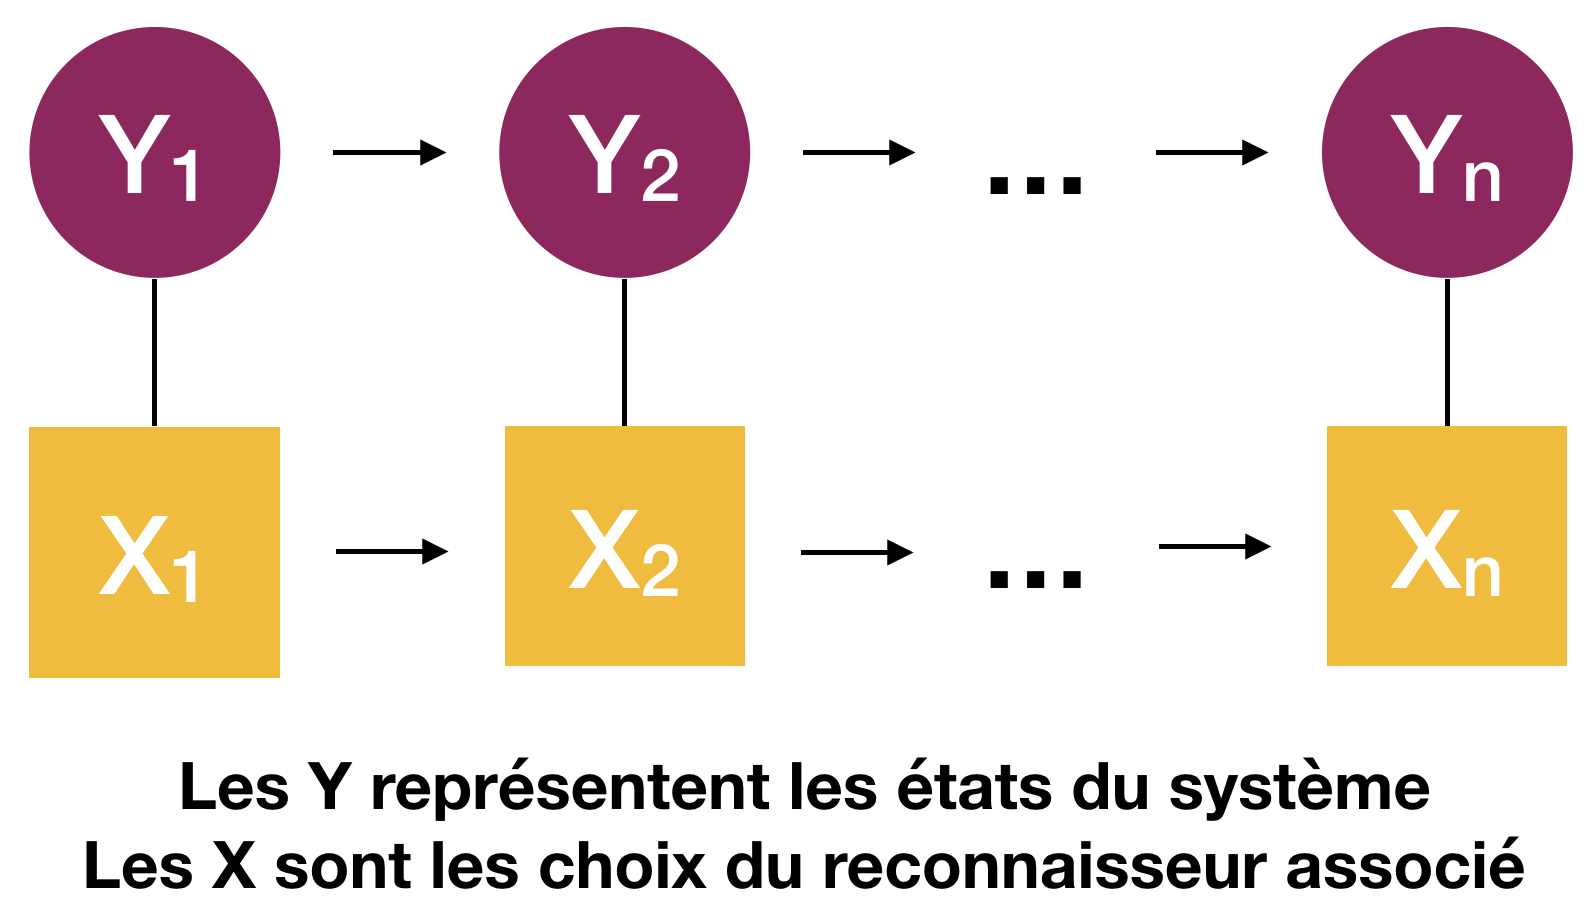
\includegraphics[width=0.6\linewidth]{mmc.png}
\end{center}
\end{mdframed}

\subsection{Champs Aléatoires Conditionnels}

Les Champs Aléatoires Conditionnels sont des modèles basés également sur des probabilités et
sur une structure similaire aux MMC. La principale différence entre ces deux méthodes est que pour les MMC,
les probabilités de choix des caractères dépendent d'un état, tandis que pour les CAC, le choix d'un
caractère peut être réalisé depuis n'importe quel état, avec une pondération par un potentiel.
Cette approche permet alors de prendre en compte l'ensemble du contexte local de la séquence observée
du fait de l'hypothèse de non-indépendance des états. Ce modèle est donc plus approprié pour l'analyse de
séquences structurées. Cependant, ils n'effectuent pas d'étiquetage de séquence lors de leur apprentissage,
et ne possèdent pas de structuration interne qui leur permettrait de saisir des structures de plus haut
niveau telles que les titres ou la date dans un document.

\paragraph{}
\begin{mdframed}[frametitle={Schéma de transition et d'observation d'un CAC}, innerbottommargin=10]
\begin{center}
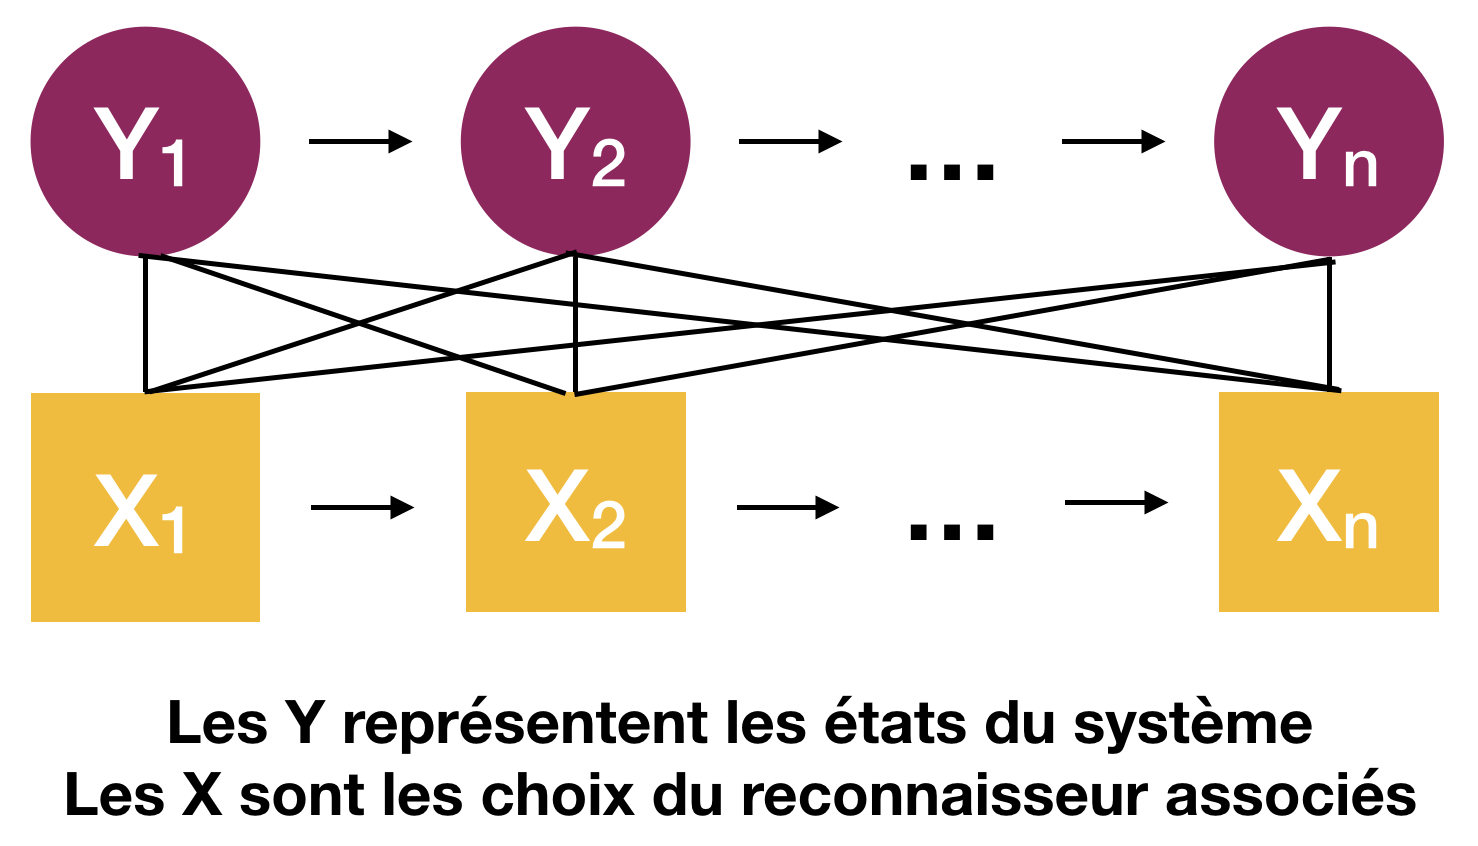
\includegraphics[width=0.6\linewidth]{cac.png}
\end{center}
\end{mdframed}

\subsection{Réseaux de Neurones Récurrents}

Les Réseaux de Neurones Récurrents sont basés sur la structure classique des réseaux de neurones,
avec une modification : chaque neurone des couches cachées possède également en entrée les sorties
des neurones correspondant à leur couche. Ceci permet d'avoir une mémoire interne des états de chaque couche.
Via cette approche, il n'est pas nécessaire d'effectuer un étiquetage des données car le réseau apprend
par lui-même. Cette méthode apporte également une vue plus globale de l'ensemble d'entrée car on ne se limite
pas à l'observation d'un état précédent. Le principal soucis de ces réseaux provient de l'apprentissage.
Ils nécessitent un grand jeu de données et on remarque une "disparition" du gradient sur les couches les plus
profondes, c'est-à-dire que les poids d'entrée ne sont que peu modifiés lors de l'apprentissage. Il faut alors
recourir à un apprentissage couche par couche, ce qui est compliqué à cause de la récurrence de ce type de réseaux.

\subsection{Réseaux de Neurones Récurrents Multi-Dimensionnels}

Les MDRNN sont conçus afin d'apporter une localité et une mémoire sur les deux dimensions de l'image traitée.
Ils sont constitués de couches de réseaux de neurones de différentes natures organisés selon l'abstraction des
données à effectuer. L'image est tout d'abord décomposée en blocs. Des réseaux récurrents la parcourent alors
en la transformant dans chaque direction diagonale. Les sorties de ces réseaux sont alors transmises à un
réseau convolutionnel qui permet d'augmenter le niveau d'abstraction des données de sortie.

\newpage

\begin{mdframed}[frametitle={Schéma de structure d'un MDRNN}, innerbottommargin=10]
\begin{center}
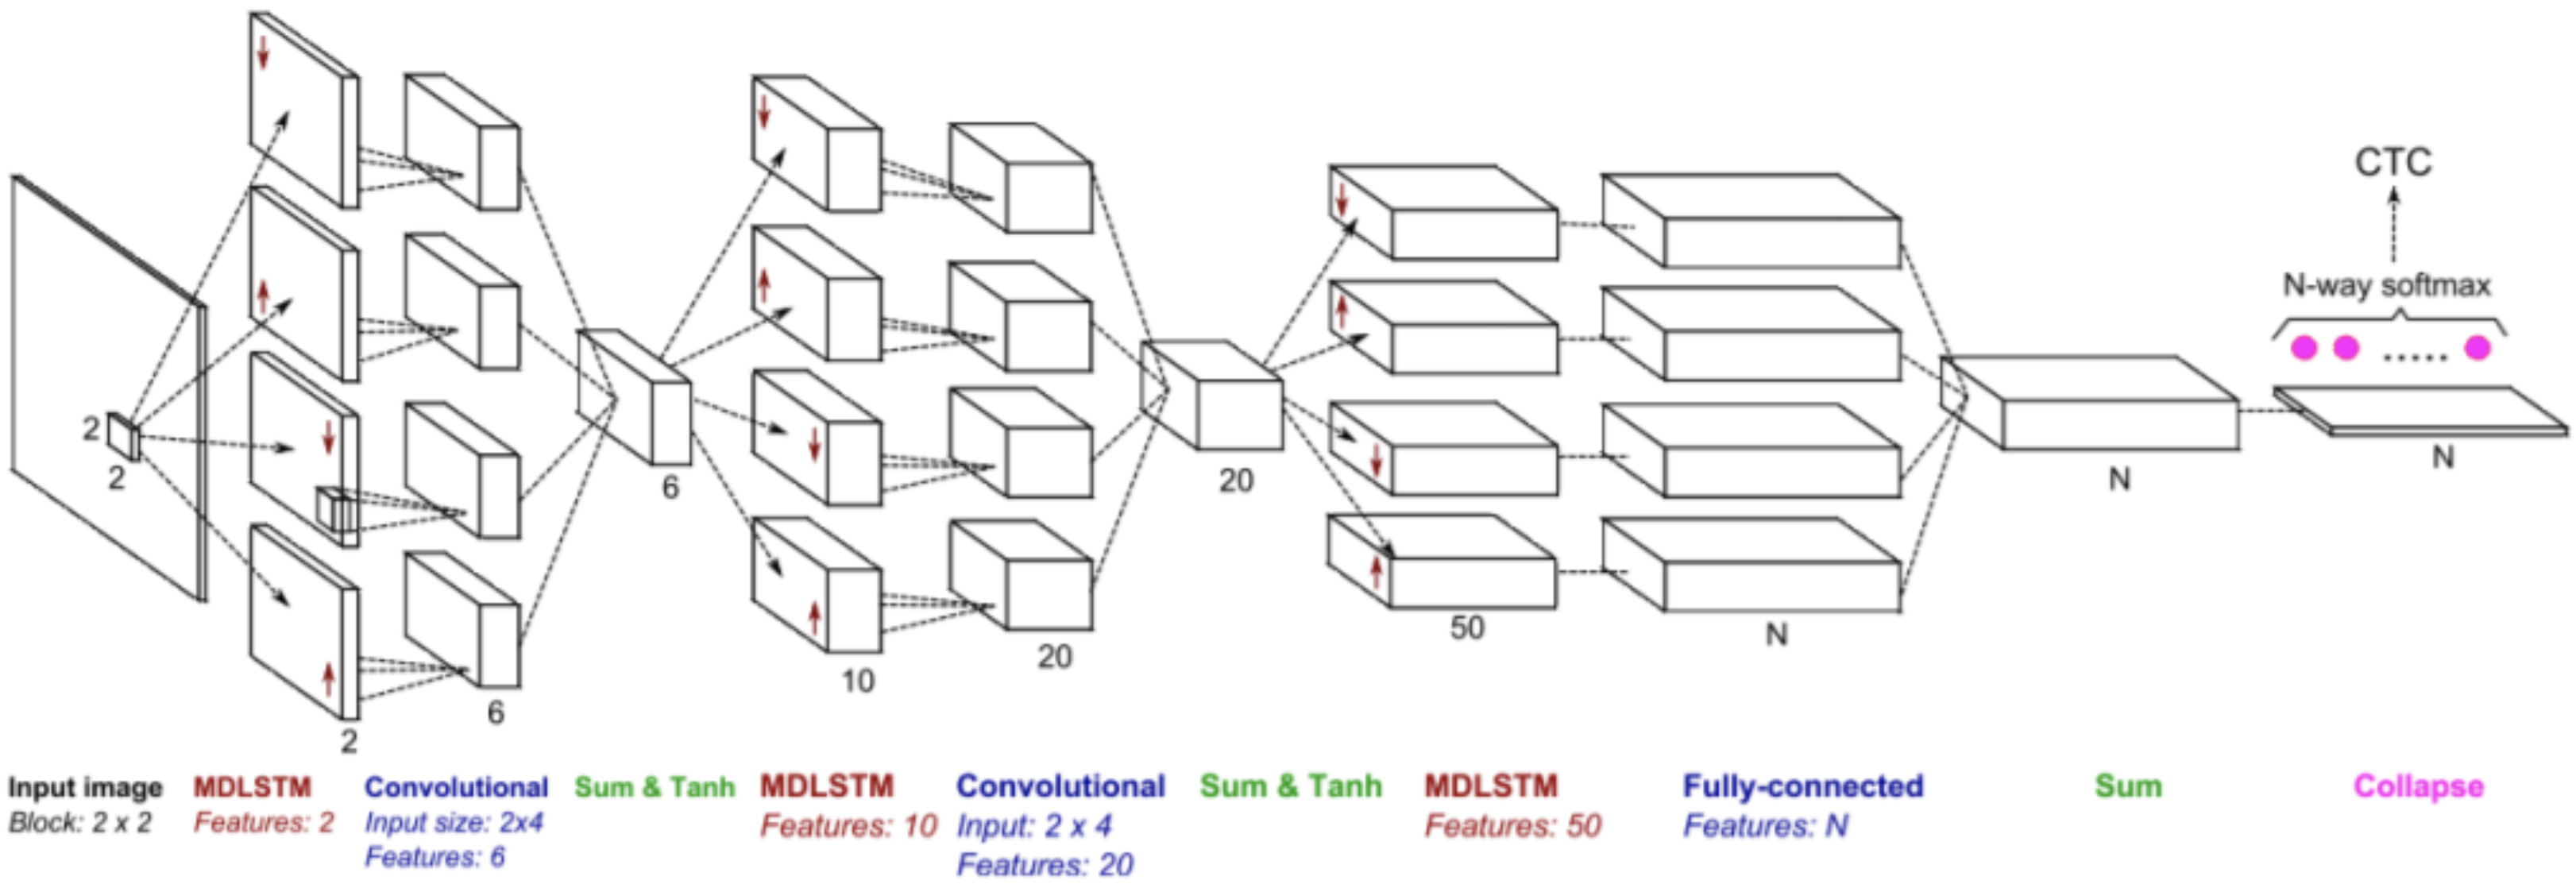
\includegraphics[width=0.6\linewidth]{mdrnn.png}
\end{center}
\end{mdframed}

\paragraph{}
Cependant, cette structure ne permet pas une segmentation de l'image de départ. Il est donc nécessaire de créer
cette segmentation afin d'établir une relation entre les données d'entrée et les sorties. Afin de réaliser cette
segmentation, une adaptation des algorithmes d'apprentissage est nécessaire.

\section{Détecteur de lignes}

Afin de pouvoir utiliser les techniques de reconnaissance manuscrite, il est d'abord nécessaire
de faire une segmentation des documents numérisés que nous possédons en entrée. La méthode
usuelle dans le domaine de la reconnaissance manuscrite est la segmentation par ligne des documents.
Pour ce faire, plusieurs techniques sont documentées dans la littérature concernant l'OCR
(\textit{Optical Character Recognition}). La segmentation en lignes est une étape importante pour
la reconnaissance manuscrite puisqu'un mauvais découpage va inévitablement poser des problèmes
lors des étapes suivantes de la reconnaissance.

\paragraph{}
Il est alors important d'identifier les problèmes que pose la détection de lignes dans les documents manuscrits.
En effet, certains aspects sont à prendre en compte :
\begin{itemize}
\item Les lignes fluctuent au sein d'un même document;
\item Les lignes d'un texte ne sont pas espacées régulièrement;
\item Certaines lignes peuvent se chevaucher;
\item L'espace interligne lui aussi peut varier d'une ligne à une autre et d'un paragraphe à un autre;
\item Les lignes d'un paragraphe peuvent avoir une courbure globale et une courbure locale propre à
chaque ligne (et même locale à une partie d'une ligne).
\end{itemize}

\paragraph{}
Tous ces paramètres pouvant différer entre deux paragraphes, deux textes, et deux écrivains. Nous allons maintenant
présenter rapidement les principales techniques documentées dans la littérature de l'OCR, pour ensuite décrire plus
précisément le fonctionnement des deux solutions fournies par IntuiDoc pour la détection des lignes d'un document manuscrit.
Il existe globalement deux types d'approches pour la détection des lignes dans un document manuscrit : les approches
descendantes et les approches ascendantes. Les approches descendantes sont basées sur la technique de la projection.
La projection horizontale est appliquée au document ou à une partie du document. Ensuite, une analyse sur les \textit{maxima},
les \textit{minima} et les composantes connexes entre deux \textit{minima} consécutifs permettent de déterminer les lignes.
Les approches ascendantes sont basées sur le bas niveau (au niveau pixel ou composantes connexes). La classification
par plus proches voisins (KNN), la transformée de Hough, la technique du lissage, et la technique de répulsif-attractif
utilisent ce type d'approches. Dans le cadre de notre projet, les algorithmes de détection des lignes nous sont
fournis par l'équipe IntuiDoc. Ils utilisent deux techniques différentes que nous allons décrire ici.

\subsection{Détection de ligne par floutage}

Cette technique utilise la combinaison de deux niveaux d'analyse de l'image. Tout d'abord, une première analyse bas niveau
de l'image floutée est réalisée, ce qui est efficace pour les images à forte densité textuelle. Ensuite, une analyse plus
haut niveau est effectuée, ce qui est efficace sur des images à faible densité textuelle. La combinaison des deux niveaux
d'analyse permet de gérer les problèmes liés à la détection de lignes dans les documents manuscrits évoqués au début de ce chapitre.
L'analyse bas niveau de l'image floutée est composée de deux étapes que sont l'extraction de régions noires dans l'image afin de
construire des parties de l'axe de la ligne, ainsi que la construction de l'axe de la ligne.

\begin{mdframed}[innerbottommargin=10]
\begin{center}
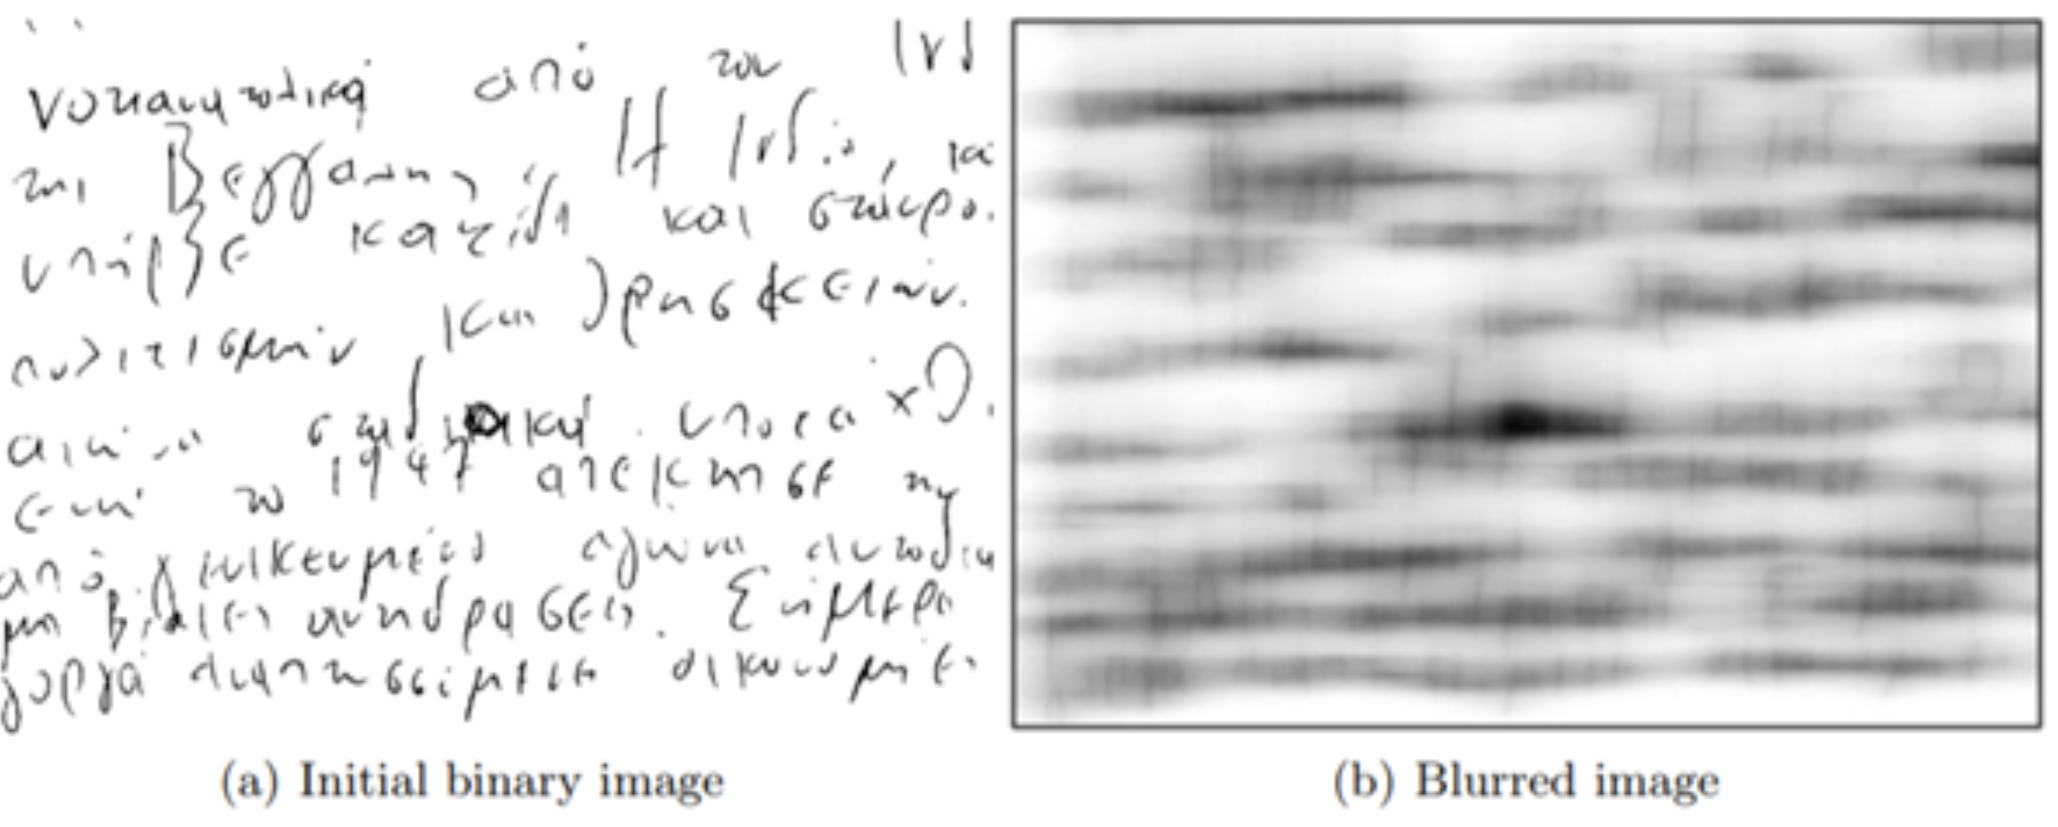
\includegraphics[width=0.6\linewidth]{detect1.png}
\end{center}
\end{mdframed}

\paragraph{}
Afin d'extraire les régions noires correspondant à des parties d'une ligne, il est nécessaire d'effectuer préalablement un
traitement sur l'image. Tout d'abord, l'image est floutée, puis une double binarisation lui est appliquée. Le résultat est
une image dans laquelle sont en évidence les « régions noires » qui vont être utilisées pour construire l'axe des lignes.

\begin{mdframed}[innerbottommargin=10]
\begin{center}
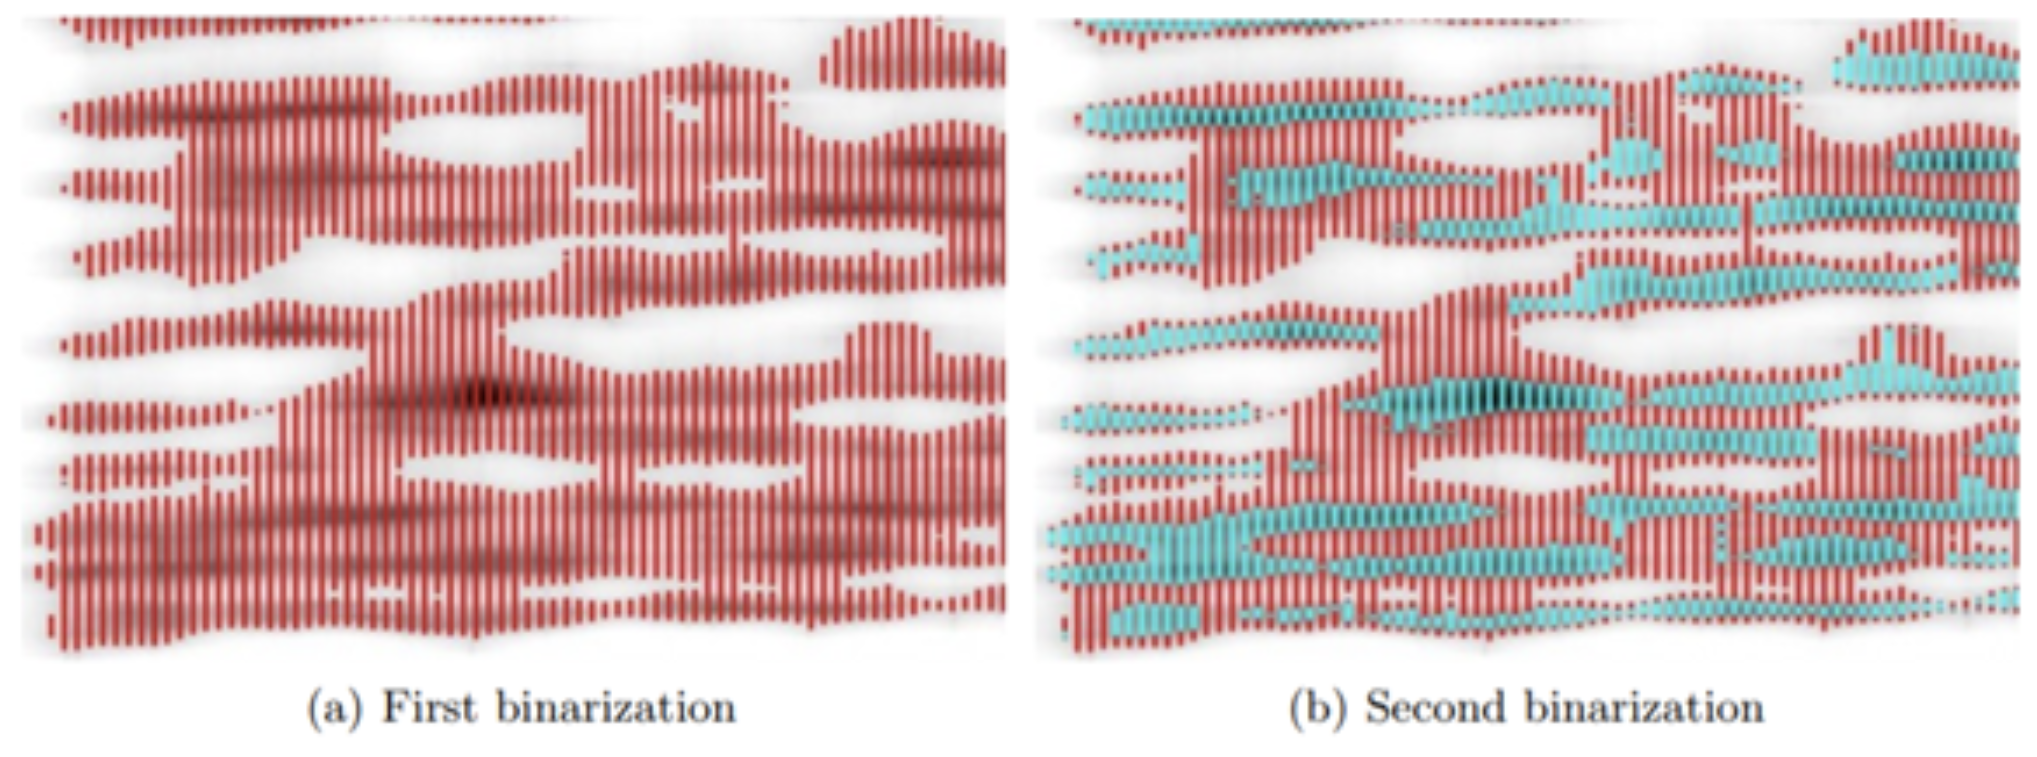
\includegraphics[width=0.6\linewidth]{detect2.png}
\end{center}
\end{mdframed}

\paragraph{}
Ces traitements d'image et la localisation de ces « zones noires » vont permettre ensuite de construire les axes des lignes.
Une analyse de la position et de l'épaisseur de ces zones va permettre de les relier entre elles. On pourra alors calculer
une épaisseur moyenne et une pente moyenne pour le document, données qui vont ensuite servir pour étendre les axes.

\begin{mdframed}[innerbottommargin=10]
\begin{center}
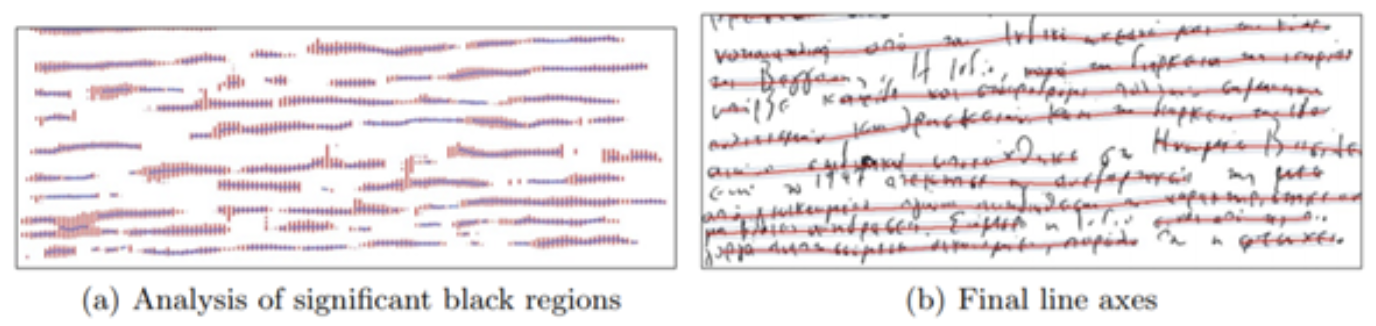
\includegraphics[width=0.6\linewidth]{detect3.png}
\end{center}
\end{mdframed}

\paragraph{}
En effet, la dernière opération de cette étape consiste à trier les différents axes créés. Des règles prenant en compte l'épaisseur,
la position et la pente des axes vont déterminer quels axes fusionner et quels axes supprimer. On peut obtenir des axes incomplets
en résultat de cette première analyse bas niveau. Cependant, aucune analyse supplémentaire ne peut être réalisée à ce niveau.

\paragraph{}
Le deuxième niveau d'analyse prend en compte le modèle du document étudié. À partir des différents axes de lignes créés dans l'étape
précédente, le but est de créer les lignes du texte. Ainsi, en fonction du document étudié, les stratégies de construction des lignes
seront différentes. Afin de spécifier un document, une description grammaticale basée sur deux types d'entités (les éléments connectés
et les axes créés précédemment) est effectuée. La description grammaticale du modèle du document va permettre de localiser les lignes
du texte et d'assigner des pixels à des lignes. Grâce à la description grammaticale et à des règles judicieusement choisies, on peut alors
construire les lignes du document. Cependant, il peut-être nécessaire (selon le domaine d'application) d'associer chaque pixel à sa ligne.
Une dernière analyse basée sur la description grammaticale du document couplée à certaines informations sur le document
est effectuée pour réaliser l'association.

\subsection{Détection de ligne par réseau de neurone à convolution}

Les réseaux de neurones à convolution comparent les images fragment par fragment et recherchent des fragments caractéristiques.
Par exemple, un réseau de neurones à convolution cherchant à déterminer si une image est un X ou pas va chercher les caractéristiques
définissant les X, les diagonales et leur entre-croisement. Lorsqu'on lui présente une image, le système ne sait alors pas si les
caractéristiques sont présentes ni leur localisation. Il va alors calculer dans toute l'image si la caractéristique est présente.
Pour compléter une convolution, on répète ce processus alignant les caractéristiques à chaque sous-partie de l'image.
Le résultat de chaque convolution est une image stockant le résultat de la comparaison, avec un 1 pour une similitude et un -1
pour une différence par exemple. Ensuite, à partir du résultat de chaque convolution, on crée un tableau situant où les
caractéristiques se trouvent dans l'image. On obtient alors des images correspondant à l'image de base découpée en filtres.
On répète le processus de convolution pour chaque caractéristique, et on obtient alors la couche de convolution.

Cependant, le nombre d'opérations augmente linéairement avec le nombre de pixels de l'image et le
nombre de pixels de chaque caractéristique. On peut alors effectuer du \textit{pooling}. On va
réduire le nombre de pixels de l'image, en passant une fenêtre de quelques pixels sur l'image,
et dans laquelle on ne garde que la valeur qui nous importe. Ainsi, le réseau ne situe pas précisément
les caractéristiques dans l'image, il connaît seulement leur présence ou non. La couche de
\textit{pooling} sert simplement à diminuer la charge de calcul. En effet, on garde le même nombre
d'images avec les mêmes informations, mais le nombre de pixels est moindre.

\section{Format de description d'image}

\subsection{GEDI}

GEDI est un outil qui permet d'annoter des documents scannés. Il est ainsi très utile pour établir
la vérité terrain. Il met en scène deux types de documents : des images qui correspondent aux documents
scannés ainsi que des documents XML au format GEDI qui permettent de stocker toutes les informations
relatives aux documents scannés. On peut alors avoir, pour chaque document scanné, des informations
relatives à la position des paragraphes, à la langue dans laquelle le texte est écrit, ou encore à
la forme du texte (manuscrit ou imprimé). La vérité terrain que nous aurons au sein de notre projet
aura été établie avec GEDI.

\subsection{PiFF}

Le Pivot File Format (PiFF) est un format de description d'image basé sur JSON et créé par différents
chercheurs français, dont notre encadrant de projet, Bertrand COÜASNON. Ce format est très utile pour l'analyse
de documents puisqu'il permet le partage de jeu de données, le traitement de résultats ainsi que
l'utilisation d'outils déjà existants sans avoir à faire de conversion entre les différents formats
qui pourraient exister. De ce fait, les différentes étapes de l'analyse de documents peuvent être effectuées
par différentes équipes sans qu'il n'y ait de conflit au niveau du format des données, ce qui permet une
collaboration plus facile. Les données présentes en entrée dans le cas de notre projet seront au format PiFF.
Par conséquent, les données après traitement par le logiciel devront également être dans ce format.